\documentclass[a4paper,12pt]{scrartcl} % From KOMA-script
\usepackage[margin=1in]{geometry}
\usepackage{ mathrsfs }
\usepackage{xcolor}
\usepackage{graphicx}
\usepackage{fancyhdr}
\usepackage{lipsum} % For filler text
\usepackage{amsthm}
\usepackage{times}
\usepackage{microtype}
\usepackage{listings}
\usepackage{amsmath, amssymb, amsfonts, amssymb, float, enumitem}
\definecolor{darkbg}{HTML}{1E1E1E}
\definecolor{darktext}{HTML}{E0E0E0}
\definecolor{theoremcolor}{HTML}{d3dce5}
\definecolor{answercolor}{HTML}{e9dfc0}
\definecolor{sectioncolor}{HTML}{dec3c3}
\pagecolor{darkbg}
\color{darktext}
\newenvironment{solution}
  {\par\color{answercolor}\textbf{Solution:}\ }
  {\par}
\newenvironment{prf}
  {\par\textbf{Proof:}\ }
  {\par}

\newcounter{customcounter}
\newcommand{\setcustomcounter}[1]{\setcounter{customcounter}{#1}}

\newtheoremstyle{darktheorem}
  {\topsep}{\topsep}
  {\itshape\color{theoremcolor}}{}
  {\bfseries\color{theoremcolor}}{.}{.5em}{}
\theoremstyle{darktheorem}
\newtheorem{theorem}{Theorem}[section]
\newtheorem{lemma}[theorem]{Lemma}
\newtheorem{proposition}[theorem]{Proposition}
\newtheorem{corollary}[theorem]{Corollary}
\newtheorem{definition}[theorem]{Definition}
\newtheorem{example}[theorem]{Example}
\newtheorem{exercise}[customcounter]{Exercise}

\usepackage{fancyhdr}
\pagestyle{fancy}
\setlist[enumerate]{label=(\alph*)}

% Clear default headers
\fancyhf{}
\renewcommand{\headrulewidth}{0pt}

% Set Author and Date in the top left
\fancyhead[L]{\textcolor{darktext}{\small Asher Christian \\ 006-150-286 \\ \today }}

\begin{document}


\title{\color{sectioncolor}HW 2 Math 151B}
\author{}
\date{}
\maketitle

% Apply fancyhdr on the title page
\thispagestyle{fancy}

\begin{exercise}
    \[
        y' = 1 \hspace{1cm} y(0) = 0
    .\] 
\end{exercise}
\begin{solution}
    \begin{enumerate}
        \item
        We have
        \[
            y_{n+1} = y_n + h \sum_{i=1}^{s}b_ik_i
        .\] 
        so it suffices to show that $k_i = 1$ for all $i$. This is true since each
        \[
        k_i = f(\hat t, \hat y)
        .\] 
        for some $\hat t, \hat y$, but since  $f(t,y) = 1$ regardless of input, this simplifies to
        \[
            k_i = 1 \hspace{1cm} \forall i
        .\] 
        \item
            consider local truncation error assuming $y_n = y(t_n)$, also note that the true solution of the equation is  $y(t) = t$
            \[
                y(t_{n+1}) - y_{n+1} = t + h - t - h \sum_{i=1}^{s}b_i
            .\] 
            \[
            = h(1-\sum_{i=1}^{s}b_i)
            .\] 
            if $\sum_{i=1}^{s}b_i = 1$ then the local truncation error is $0$ which is $O(h^2)$ but if $\sum_{}^{}b_i \ne 1$ then the LTE is $O(h)$.
    \end{enumerate}
\end{solution}
\begin{exercise}
    \[
        u(t) = t \hspace{1cm} v(t) = y
    .\] 
\end{exercise}
\begin{solution}
    \begin{enumerate}
        \item 
            \[
                K_{i_2} = F(Y_n + h \sum_{j=1}^{s}a_{i,j}K_j)_{2}
            .\] 
            Note that if $K_{i,n} = \begin{pmatrix} a \\ b \end{pmatrix} $ that $a = 1$ since $F(\begin{pmatrix} a \\ b \end{pmatrix} ) = \begin{pmatrix} 1 \\ c \end{pmatrix} $ for some $c$.
            \[
            Y_n = \begin{pmatrix} u_n \\ v_n \end{pmatrix} 
            .\] 
            \[
                Y_n + h \sum_{j=1}^{s}a_{i,j}K_j = \begin{pmatrix} u_n \\ v_n \end{pmatrix} + h \sum_{j=1}^{s}a_{i,j}\begin{pmatrix} 1 \\ K_{j,2} \end{pmatrix} 
            .\] 
            in particular the first component of this calculation is $u_n + ha_{i,j}$ so
            \[
                F(Y_n + h \sum_{j=1}^{s}a_{i,j}K_j)_2 = f(u_n + h\sum_{j=1}^{s}a_{i,j}, v_n + h \sum_{j=1}^{s}a_{i,j}K_{j,2})
            .\] 
            as described.
        \item Expanding the second variable of the expression given in (6) we get
            \[
                v_{n+1} = v_n + h \sum_{i=1}^{s}b_i f(u_n + h\sum_{j=1}^{s}a_{i,j}, v_n + h \sum_{j=1}^{s}a_{i,j}K_{j,2})
            .\] 
        \item we have
            \[
                y_{n+1} = y_n + h \sum_{i=1}^{s}b_if(t_n + c_ih, y_n + h\sum_{j=1}^{s}a_{i,j}k_j)
            .\] 
            equating this equation with the previous shows that we must have
            \[
                c_i = \sum_{j=1}^{s}a_{i,j}
            .\] 
    \end{enumerate}
\end{solution}
\begin{exercise}
    \[
        \mu = 0.012277471 \hspace{1cm} \mu_0 = 1-\mu
    .\] 
    \[
    x'' = 2y' + x - \frac{\mu_0(x+\mu)}{r_1^{3}} - \frac{\mu(x-\mu_0)}{r_2^{3}}
    .\] 
    \[
    y'' = -2x' + y - \frac{\mu_0y}{r_1^{3}} - \frac{\mu y}{r_2^{3}}
    .\] 
    \[
    r_1 = \sqrt{(x+\mu)^2 + y^2}
    .\] 
    \[
    r_2 = \sqrt{(x-\mu_0)^2 + y^2}
    .\] 
\end{exercise}
\begin{solution}
    \begin{enumerate}
        \item
            this system is equivalent to 
            \[
            \begin{pmatrix} x \\ x' \\ y \\ y' \end{pmatrix}' = \begin{pmatrix} x' \\ 2y' + x - \frac{\mu_0(x+\mu)}{r_1^{3}} - \frac{\mu(x-\mu_0)}{r_2^{3}} \\ y' \\ -2x' + y - \frac{\mu_0y}{r_1^{3}} - \frac{\mu y}{r_2^{3}} \end{pmatrix} 
            .\] 
        \item 
            \begin{lstlisting}
import numpy as np
import matplotlib.pyplot as plt

def velocity_field(t, y):
    """
    Compute the velocity field for the restricted three-body problem.

    Parameters:
        t : float
            Time (not used explicitly here since the system is autonomous).
        y : ndarray
            4D vector: [x, x_dot, y, y_dot]

    Returns:
        f : ndarray
            4D vector of derivatives [x_dot, x_ddot, y_dot, y_ddot]
    """
    mu = 0.012277471
    mu0 = 1 - mu

    x, x_dot, y_pos, y_dot = y

    r1 = np.sqrt((x + mu)**2 + y_pos**2)
    r2 = np.sqrt((x - mu0)**2 + y_pos**2)

    f = np.zeros(4)
    f[0] = x_dot
    f[1] = 2*y_dot + x - (mu0 * (x + mu)) / r1**3 - (mu * (x - mu0)) / r2**3
    f[2] = y_dot
    f[3] = - 2*x_dot + y_pos - (mu0 * y_pos) / r1**3 - (mu * y_pos) / r2**3

    return f

# Initial condition
y0 = np.array([0.994, 0.0, 0.0, -2.00158510637908252240537862224])

# Simulation parameters
T = 17.1
N = 10000  # You can adjust this
tvec = np.linspace(0, T, N)
h = tvec[1] - tvec[0]

# Storage for results
y_stored = np.zeros((4, N))
y = y0.copy()

for n in range(N):
    t = tvec[n]

    # RK4 method
    k1 = velocity_field(t, y)
    k2 = velocity_field(t + h/2, y + h/2 * k1)
    k3 = velocity_field(t + h/2, y + h/2 * k2)
    k4 = velocity_field(t + h, y + h * k3)

    y += (h/6) * (k1 + 2*k2 + 2*k3 + k4)
    y_stored[:, n] = y

# Plotting the results
mu = 0.012277471
mu0 = 1 - mu

plt.figure(figsize=(8, 6))
plt.plot(mu, 0, 'ro', markersize=8, label='Planet A')
plt.plot(mu0, 0, 'bo', markersize=8, label='Planet B')
plt.plot(y_stored[0, :], y_stored[2, :], 'k-', linewidth=1.5, label='Trajectory')
plt.xlabel('x')
plt.ylabel('y')
plt.title('Trajectory of the planet using 4 step RK')
plt.legend()
plt.grid(True)
plt.tight_layout()
plt.savefig("path.png")
plt.show()
            \end{lstlisting}
        \item it takes approximately 10000 uniform steps to resolve the dynamics propertly.\\
            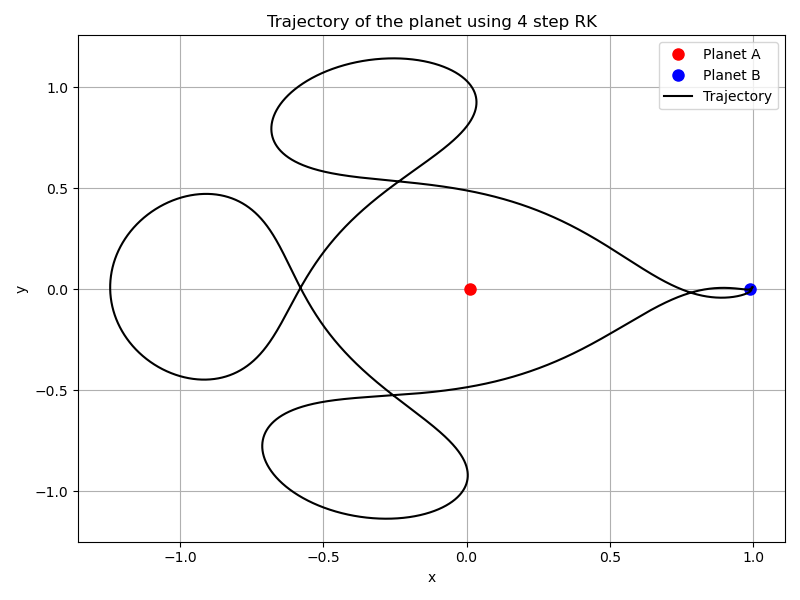
\includegraphics[width = \textwidth]{path.png}
        \item 
            \begin{lstlisting}
T = 17.1
y0 = np.array([0.994, 0.0, 0.0, -2.00158510637908252240537862224])
out = scipy.integrate.solve_ivp(velocity_field, (0,T),y0,'RK45',rtol = 1e-6)

mu = 0.012277471
mu0 = 1 - mu

plt.figure(figsize=(8, 6))
plt.plot(mu, 0, 'ro', markersize=8, label='Planet A')
plt.plot(mu0, 0, 'bo', markersize=8, label='Planet B')
plt.plot(out.y[0], out.y[2], 'k-', linewidth=1.5, label='Trajectory')
plt.xlabel('x')
plt.ylabel('y')
plt.title('Trajectory of the planet using ODE solver RK45')
plt.legend()
plt.grid(True)
plt.tight_layout()
plt.savefig("ode45.png")
plt.show()
print(len(out.t))

            \end{lstlisting}
            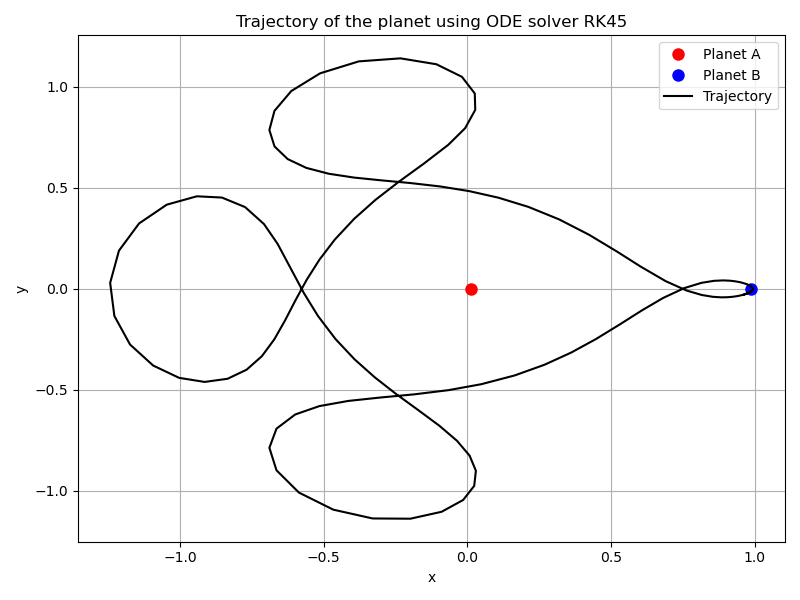
\includegraphics[width = \textwidth]{ode45.png}
            I chose relative error tolerance of 10e(-6) which resulted in 146 times steps. But i noticed that leaving the error tolerance 
            at 10e(-3) is sufficient to trace the general shape, but the output is more choppy.
            This method took significantly fewer steps than my own method to achieve the accurate spacing.
    \end{enumerate}
\end{solution}

\begin{exercise}
    \[
        y(t_{n+1}) - y(t_n) = \int_{t_n}^{t_{n+1}} y'(t)dt
    .\] 
\end{exercise}
\begin{solution}
    \begin{enumerate}
        \item given the three points the the lagrange polynomial is given by
            \[
                p(t) = \frac{(t-t_n)(t-t_{n+1})}{(t_{n-1}-t_n)(t_{n-1}-t_{n+1})}y'(t_{n-1}) + \frac{(t-t_{n-1})(t-t_{n+1})}{(t_n - t_{n-1})(t_n-t_{n+1}}y'(t_n) + \frac{(t-t_{n-1})(t-t_n)}{(t_{n+1}-t_{n-1})(t_{n+1}-t_n)}y'(t_{n+1})
            .\] 
            \[
                p(t) = \frac{(t-t_n)(t-t_{n+1})}{(h)(2h)}y'(t_{n-1}) + \frac{(t-t_{n-1})(t-t_{n+1})}{(h)(-h)}y'(t_n) + \frac{(t-t_{n-1})(t-t_n)}{(2h)(h)}y'(t_{n+1})
            .\] 
            \[
                p(t) = \frac{y'(t_{n-1})}{2h^2}(t-t_n)(t-t_{n+1}) - \frac{y'(t_n)}{h^2}(t-t_{n-1})(t-t_{n+1}) + \frac{y'(t_{n+1})}{2h^2}(t-t_{n-1})(t-t_n)
            .\] 
        \item 
            \[
                \int_{t_n}^{t_{n+1}}(t-t_n)(t-t_{n+1})dt = h\int_{0}^{1}(sh)(sh - h)ds =  h^3\int_{0}^{1}(s)(s-1)ds = -\frac{h^{3}}{6}
            .\] 
            \[
                \int_{t_n}^{t_{n+1}}(t-t_{n-1})(t-t_{n+1})dt = h\int_{0}^{1}(sh+h)(sh-h)ds = h^{3}\int_{0}^{1}(s^2-1)ds = -\frac{2h^{3}}{3}
            .\] 
            \[
                \int_{t_n}^{t_{n+1}}(t-t_{n-1})(t-t_{n})dt = h\int_{0}^{1}(sh+h)(sh)ds = h^{3}\int_{0}^{1}(s^2+s)ds = \frac{h^{3}5}{6}
            .\] 
        \item 
            \[
                \int_{t_n}^{t_{n+1}}p(t)dt =  \frac{y'(t_{n-1})}{2h^2}\int_{t_n}^{t_{n+1}}(t-t_n)(t-t_{n+1})dt - \frac{y'(t_n)}{h^2}\int_{t_n}^{t_{n+1}}(t-t_{n-1})(t-t_{n+1})dt
            .\] 
            \[
                + \frac{y'(t_{n+1})}{2h^2}\int_{t_n}^{t_{n+1}}(t-t_{n-1})(t-t_n)dt
            .\] 
            \[
                = h(y'(t_{n-1})(-\frac{1}{12}) - y'(t_n)(-\frac{2}{3}) + y'(t_{n+1}) \frac{5}{12}) 
            \]
            \[
                = h(\frac{5}{12}f(t_{n+1},y(t_{n+1})) + \frac{8}{12}f(t_n,y(t_n)) - \frac{1}{12}f(t_{n-1},y(t_{n-1})))
            .\] 
        \item we previously stated that $y(t_{n+1})- y(t_n) \approx \int_{t_n}^{t_{n+1}}p(t)dt = h(\frac{5}{12}f(t_{n+1},y(t_{n+1})) + \frac{8}{12}f(t_n,y(t_n)) - \frac{1}{12}f(t_{n-1},y(t_{n-1})))$
            Thus we get the method
            \[
                y_{n+1} = y_n + h(\frac{5}{12}f_{n+1})) + \frac{8}{12}f_n - \frac{1}{12}f_{n-1})
            .\] 
            shifting we get
            \[
                y_{n+2} = y_{n+1} + h(\frac{5}{12}f_{n+2} + \frac{8}{12}f_{n+1} - \frac{1}{12}f_n)
            .\] 
            The local truncation error is
            \[
                \tau = y(t_n + 2h) - y(t_n + h) - h(\frac{5}{12}f_{n+2} + \frac{8}{12}f_{n+1} - \frac{1}{12}f_n)
            .\] 
            where here we say that $f_{t_n} = f(t_n, y(t_n))$ in shorthand\\
            taylor expanding about $t_n$ we get
             \[
            y(t_n+2h) = y + 2hy' + 2h^2y'' + \frac{(2h)^{3}}{3!}y^{(3)} + O(h^{4})
            .\] 
            \[
            y(t_n + h) = y + hy' + \frac{h^2}{2}y'' + \frac{h^{3}}{3!}y^{(3)} + O(h^{4})
            .\] 
            so we get
            \[
                \tau = hy' + \frac{3}{2}h^2y'' + \frac{7}{6}h^{3}y^{(3)} - h(\frac{5}{12}y'(t_n+2h) + \frac{8}{12}y'(t_n+h) - \frac{1}{12}y') + O(h^{4})
            .\] 
            expanding further we get
            \[
            y'(t_n + 2h) = y' + 2hy'' + 2h^2y^{(3)} + O(h^{3})
            .\] 
            \[
            y'(t_n + h) = y' + hy'' + \frac{h^2}{2}y^{(3)} + O(h^{3})
            .\] 
            substituting we get
            \[
                \tau = hy' + \frac{3}{2}h^2y'' + \frac{7}{6}h^{3}y^{(3)} - \frac{5}{12}hy' - \frac{5}{6}h^2y'' - \frac{5}{6}h^{3}y^{3} - \frac{8}{12}hy' - \frac{8}{12}h^2y'' - \frac{4}{12}h^{3}y^{(3)} + \frac{1}{12}hy' + O(h^{4})
            .\] 
            group like terms we get
            \[
            \tau = hy'(1 - \frac{5}{12} - \frac{8}{12} + \frac{1}{12}) + h^2t''(\frac{3}{2} - \frac{5}{6} - \frac{4}{6}) + h^{3}y^{(3)}(\frac{7}{6} - \frac{5}{6} - \frac{2}{6}) + O(h^{4})
            .\] 
            \[
            \tau = O(h^{4})
            .\] 
            thus this method is third order accurate
    \end{enumerate}
\end{solution}
\begin{exercise}
    
\end{exercise}
\begin{solution}
    Recall backward euler
    \[
        y_{n+1} = y_n + hf(t_{n+1},y_{n+1})
    .\] 
    which is equivalent to
    \[
        y_{n+1} - y_n - hf(t_{n+1},y_{n+1}) = 0
    .\] 
    thus
    \[
        \mathcal{L}_hy(t) = y(t_n + h) - y(t_n) - hf(t_n + h, y(t_n + h))= y(t_n + h) -y(t_n) - hy'(t_n + h)
    .\] 
    we have
    \[
    y(t_n) = y(t_n + h) - hy'(t_n + h) + O(h^2)
    .\] 
    plugging in we get
    \[
        \mathcal{L}_hy(t) = y(t_n + h) - y(t_n + h) + hy'(t_n+h) - hy'(t_n + h) + O(h^2)
    .\] 
    \[
     = O(h^2)
    .\] 
    and thus BE is first order accurate.
\end{solution}
\begin{exercise}
\end{exercise}
\begin{solution}
    \begin{enumerate}
        \item I thought that the dynamic step size was coool and it was surprising how many fewer timesteps the dynamic
            approach was compared to fixed size. Maybe implementing something similar would be cool from scratch.
        \item So far everything seems pretty strraightforward, but as I mentioned last time I would appreciate more intuition behind
            the connection between LTE and accuracy, ideally proven.
        \item Overall the class is going very well, I really like the teaching style and the choice of homework problems.
    \end{enumerate}
\end{solution}

\end{document}

